\chapter{Pronghorn Model Verification}
\label{sec:vv}

The use of computational models to predict reactor response to nominal and off-normal conditions requires high software quality and a strong \gls{vv} base. The integrated documentation, use of version control systems, and \gls{ci} testing discussed in Section \ref{sec:software} ensure high software reliability, efficiency, and maintainability. Equally important is the establishment of a set of verification tests and validation benchmarks relevant to the software's intended application space. 

Efforts underway at \gls{inl} and \gls{ucb} focus on building a comprehensive software test matrix to support qualification of Pronghorn for single-phase \gls{pbr} simulations. The objective of this section is to describe a small subset of these verification tests in order to 1)~emphasize the rigor in the numerical implementation of the models in Chapter \ref{sec:PhysicalModels} and 2)~support the application of Pronghorn to low-speed gas-cooled pebble experiments in Chapter \ref{sec:sana} and to salt-cooled \glspl{pbr} in Chapter \ref{sec:pbfhr}. Additional verification exercises such as the code-to-code \gls{oecd} \gls{pbmr} benchmark and code-to-code comparisons against STAR-CCM+ are described at length elsewhere \cite{balestra,lee_2020}.

This chapter is organized as follows. Section \ref{sec:mms} discusses the use of the \gls{mms} to verify correct source implementation of all kernels and \glspl{bc}. The rigorous developer-imposed requirement to satisfy theoretical convergence rates for all source objects reflects the high caliber of the physics implementation, an essential first step before conducting more complex analyses.

The focus of Chapters \ref{sec:sana} and \ref{sec:pbfhr} are on porous flows, but the pebble region of most \glspl{pbr} is adjacent to a non-porous, open plenum that falls under the purview of a multidimensional \gls{th} core simulator such as Pronghorn. Therefore, \gls{th} models of \glspl{pbr} must be able to accurately predict fluid mixing in this plenum region and the resulting thermal stresses on core structural materials. The macroscale models derived in Chapter \ref{sec:PhysicalModels} reduce to equations applicable to open flows by setting \(\epsilon=1\), \(W=0\), \(\tilde{\mu}=\mu_f\), \(\alpha=0\), \(\kappa_f=k_f\), and \(\kappa_s=k_s\). To contrast with the porous simulations in Chapters \ref{sec:sana} and \ref{sec:pbfhr} and to verify the macroscale models for open flows such as in plena, Sections \ref{sec:natural_convection} and \ref{sec:potential_flow} demonstrate application of the porous macroscale models to open flows with thermal and flow characteristics relevant to \glspl{pbr}.

Section \ref{sec:natural_convection} presents Pronghorn simulations of a numerical benchmark defined by de Vahl Davis and Jones for viscous natural convection flow in a square enclosure \cite{davis}. Many \gls{pbr} designs incorporate natural convection cooling in shutdown conditions, and this benchmark is an indication of the macroscale model's capabilities for modeling thermally-driven natural convection.

Section \ref{sec:potential_flow} presents Pronghorn simulations of inviscid flow over a cylinder. Most gas-cooled \glspl{pbr} operate at high Reynolds number, making inviscid flow models a reasonable simplification over viscous models and their accompanying boundary layer meshing requirements. In the limit of zero Mach number, the compressibility effects in the macroscale model become insignificant, allowing a comparison to the analytic incompressible potential flow solution for inviscid cylinder flow. This analysis therefore serves as a demonstration of the macroscale model's capabilities for modeling inviscid flow and compressibility effects that may be quite significant in gas-cooled systems with large core temperature rises \cite{martineau}.

All of the analyses in Chapters \ref{sec:sana} and \ref{sec:pbfhr} use the friction-dominated macroscale model in Eq.\ \eqref{eq:PrimitiveEqns} due to its more robust convergence properties and faster runtime relative to the Navier-Stokes model in Eq.\ \eqref{eq:PorousEquations}. The verification tests presented in Sections \ref{sec:natural_convection} and \ref{sec:potential_flow} therefore provide a diversity to the macroscale model applications in this dissertation and demonstrate Pronghorn's capacity as a general-purpose flow solver.

To enable reproduction of the simulations presented in this chapter, Appendix \ref{sec:reproducibility} lists all data and input files related to this chapter.

\section{Method of Manufactured Solutions}
\label{sec:mms}

The \gls{mms} is used to verify correct source code implementation of all contributions to the residuals in Eqs.\ \eqref{eq:PronghornEquations_V2WeakForm} and \eqref{eq:PrimitiveWeakForms}\mdash that is, all kernels and \gls{bc} objects.

A user-specified solution to a particular governing equation is ``manufactured'' by adding an appropriate forcing term to that equation \cite{roache}. For example, the diffusion equation with unity diffusivity has the strong form

\begin{equation}
\label{eq:diff_example}
-\nabla^2\Phi=0\ ,
\end{equation}
 
\noindent where \(\Phi\) is the solution variable. For a manufactured solution of the form

\begin{equation}
\label{eq:mms_soln}
\Phi=f(\vec{x},t)\ ,
\end{equation}

\noindent where \(f\) is a generic function, solution of the modified equation

\begin{equation}
-\nabla^2\Phi=-\nabla^2f(\vec{x},t)
\end{equation}

\noindent with the appropriate \glspl{bc} on \(\Phi\) will return the manufactured solution in Eq.\ \eqref{eq:mms_soln} provided the source implementation of the diffusion kernel is correct. Successively refining the mesh and/or time resolution can then be used to estimate convergence rates for various \gls{fe} basis function orders and \gls{fd} time integration schemes.

To verify spatial convergence, the L$^2$ norm relative to the manufactured solution is computed on a series of uniformly refined meshes. When measured in the L$^2$ norm, the \gls{fem} is second-order accurate in space with linear elements and third-order accurate in space with quadratic elements. 

While arbitrary manufactured solution spatial dependencies are selected for the spatial convergence tests, the temporal convergence tests manufacture solutions that are separable in time and space. Further, the spatial dependence is linear such that the use of linear \gls{fe} basis functions nearly isolates the time discretization error from the spatial discretization error. To verify temporal convergence, the spatial mesh is fixed and the L$^2$ norm relative to the manufactured solution is computed on a series of uniformly refined time step sizes. When measured in the L$^2$ norm, the time integration is first-order accurate in time with the backward Euler method and second-order accurate in time with the \gls{bdf2}, Crank-Nicolson, and \gls{dirk} methods. 

Correct source implementation is inferred by achieving these theoretical spatial and temporal convergence rates. As an example, \gls{mms} convergence rates for the (a) \(-\nabla\cdot(\kappa_s\nabla T_s)\) kernel and (b) \(\epsilon\rho_fC_{p_f}\partial T_f/\partial t\) kernel are shown in Fig.\ \ref{fig:convergence}. The expected convergence rates of 2 and 3 for linear and quadratic elements, respectively, are obtained for the spatial kernel. The expected convergence rates of 1 and 2 are obtained for the various time discretization schemes for the time-dependent kernel.

\begin{figure}[!h]
\centering
    \begin{subfigure}{0.48\linewidth}
        \centering
        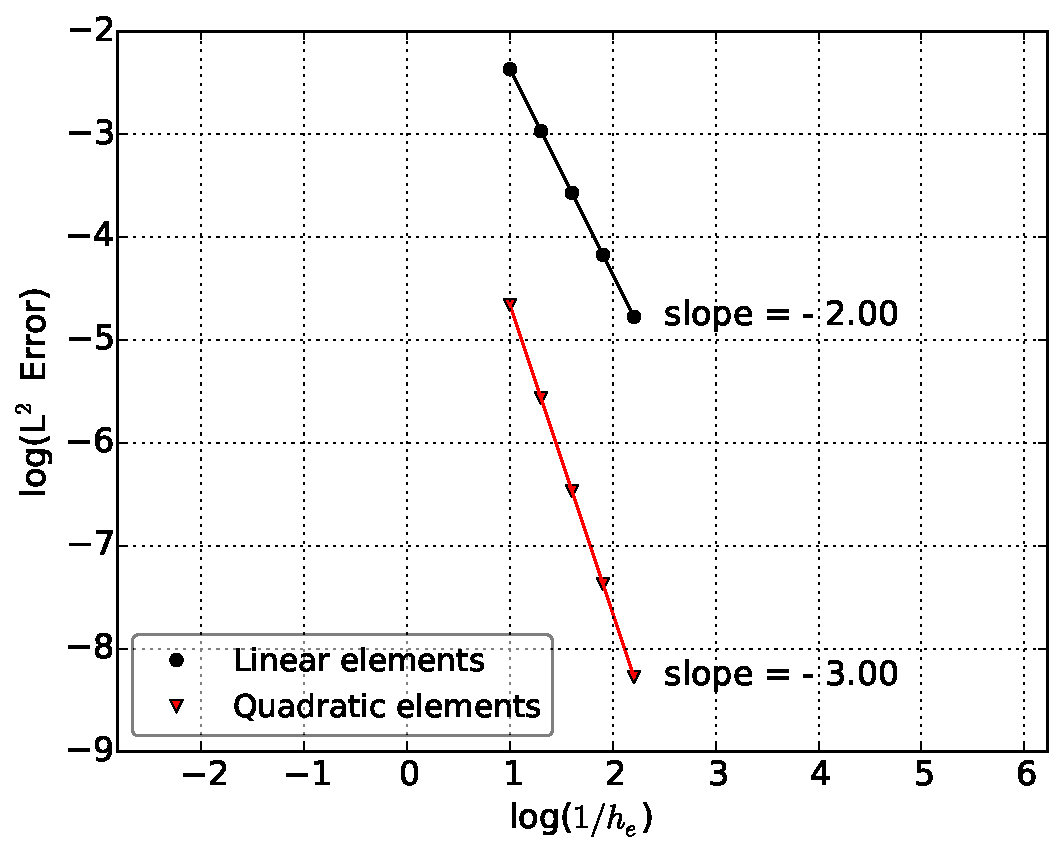
\includegraphics[width=1.0\linewidth]{figs/convergence_solid_energy_diffusion.pdf}
       \caption{\gls{mms} test of \(-\nabla\cdot \left(\kappa_s\nabla T_s\right)\)}
    \end{subfigure}
    \begin{subfigure}{0.48\linewidth}
        \centering
        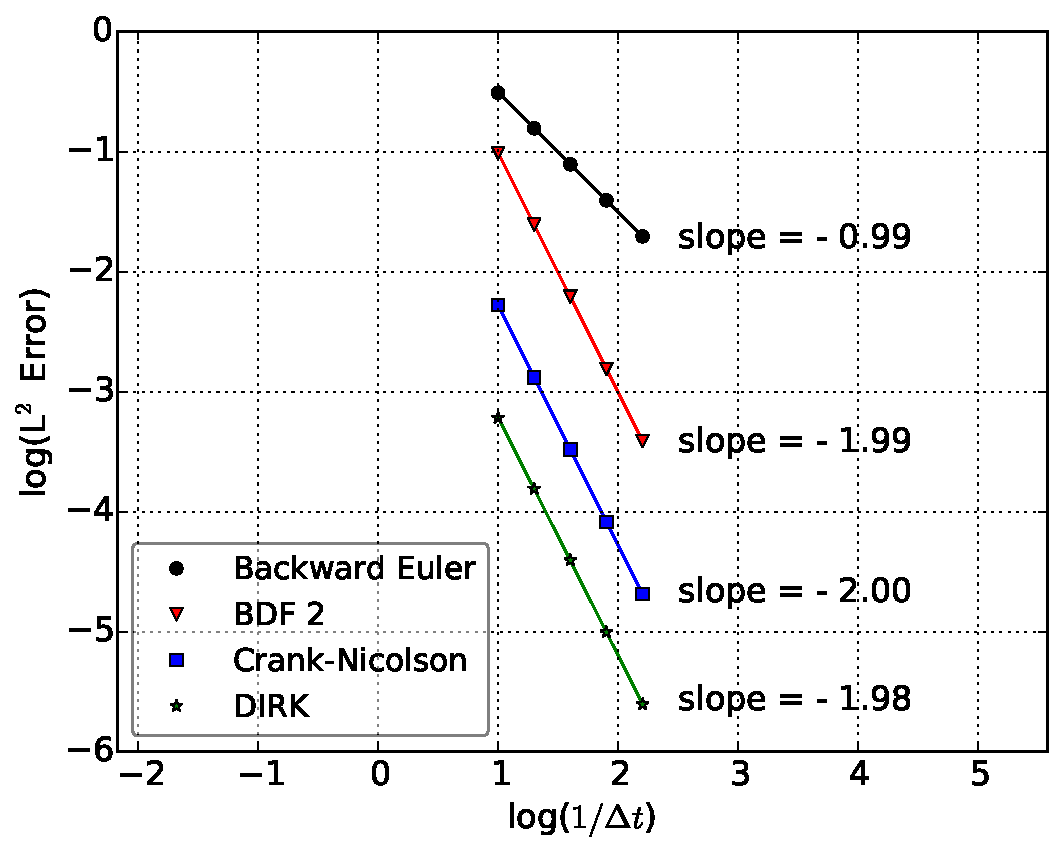
\includegraphics[width=1.0\linewidth]{figs/convergence_fluid_energy_time.pdf}
        \caption{\gls{mms} test of \(\epsilon\rho_fC_{p_f}\frac{\partial T_f}{\partial t}\)}
    \end{subfigure}
    \caption{\gls{mms} convergence studies for the (a) \(\nabla\cdot(\kappa_s\nabla T_s)\) kernel and (b) \(\epsilon\rho_fC_{p_f}\partial T_f/\partial t\) kernel. Discrete points are error measurements and solid lines are linear fits.}
    \label{fig:convergence}
\end{figure}

\section{Natural Convection in an Open Cavity}
\label{sec:natural_convection}

Many \glspl{pbr} are designed to remove decay heat via thermally-driven natural convection. The Rayleigh number \(Ra\) quantifies the relative importance of buoyant forces to diffusive forces, and is defined as

\beq
\label{eq:RaDef}
Ra\equiv\frac{|g|\rho_f^2C_{p,f}\beta_f L^3\Delta T_f}{\mu_f k_f}\ ,
\eeq

\noindent where \(\Delta T/L\) is the imposed temperature gradient in a domain of length \(L\). Provided the imposed temperature gradient is not entirely aligned with the gravitational acceleration vector, then for sufficiently large Rayleigh number, buoyant forces overcome dissipative forces to produce convective motions \cite{manneville,sandberg}.

This section presents Pronghorn simulations of flow in an open square cavity with differentially heated walls to verify the applicability of the Navier-Stokes macroscale model to open natural convection flows. This verification exercise is relevant to the use of coarse mesh tools for prediction of mixing and thermal striping in the open plena adjacent to many \gls{pbr} beds. Additional objectives of this analysis are to 1)~illustrate the reduction of the macroscale models in Chapter \ref{sec:PhysicalModels} to the open flow equations through proper selection of the macroscale closures and 2)~demonstrate mesh refinement studies for a physics simulation that are omitted in all later chapters for brevity.

The problem geometry is shown in Fig.\ \ref{fig:rb_cell}; the domain and \glspl{bc} are selected based on a benchmark defined by de Vahl Davis and Jones \cite{davis}. The cavity dimension \(L\) is 1 \si{\meter}, gravity acts in the \(-z\) direction, velocity satisfies no-slip \glspl{bc} on all surfaces, and the top and bottom boundaries are insulated. The temperature is \(T_H\) on the heated boundary and \(T_C\) on the cooled boundary. The fluid is modeled with the Navier-Stokes macroscale model in Eq.\ \eqref{eq:PorousEquations} with \(\epsilon=1\), \(W=0\), \(\tilde{\mu}=\mu_f\), \(\alpha=0\), \(\kappa_f=k_f\), and \(\kappa_s=k_s\) and properties closed by the ideal gas \gls{eos}. The Prandtl number is fixed at 0.71 and the Rayleigh number is varied from \(10^3\) to \(10^6\) by varying the fluid dynamic viscosity and thermal conductivity.

\begin{figure}[!h]
\centering
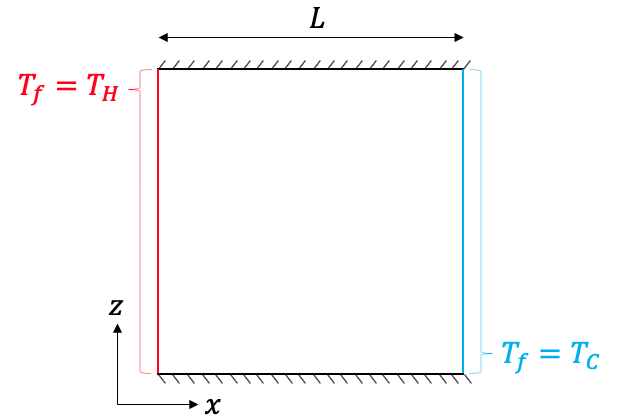
\includegraphics[width=0.5\linewidth]{figs/rb_cell.png}
\caption{Problem set-up for natural convection flow in an \(L\times L\) \si{\meter} square enclosure.}
\label{fig:rb_cell}
\end{figure}

Pronghorn predictions of velocity, temperature, and Nusselt number are compared with a reference solution distributed with the benchmark \cite{davis}. In addition to spatial velocity and temperature distributions, pointwise information requested of the original benchmark participants includes

\begin{itemize}
\itemsep0em
\item Maximum \(x\)-direction velocity on the \(x^+=0.5\) plane, \(V^+_{x,\text{max}}\), and its \(z\)-location \(z^+_u\);
\item Maximum \(y\)-direction velocity on the \(z^+=0.5\) plane, \(V^+_{z,\text{max}}\), and its \(x\)-location \(x^+_v\);
\item Maximum Nusselt number on the \(x^+=0\) plane, \(Nu_\text{max}\), and its location \(z^+_\text{max}\);
\item Minimum Nusselt number on the \(x^+=0\) plane, \(Nu_\text{min}\), and its location \(z^+_\text{min}\); and
\item Average Nusselt number \(\la Nu\ra\).
\end{itemize}

All locations, velocities, and temperatures are presented in nondimensional form by defining the following quantities,

\beq
\label{eq:nondim_x}
x^+=\frac{x}{L},\quad z^+=\frac{z}{L},\quad V_i^+=V_i\frac{\rho_f C_{p,f}L}{k_f},\quad T_f^+=\frac{T_f-T_C}{T_H-T_C}\ .
\eeq

\noindent A mesh refinement study based on a subset of the numeric information requested of benchmark participants is shown in Fig.\ \ref{fig:mr}. For each Rayleigh number, the same starting mesh is uniformly refined until the L$^1$ norm of the error in each of the scalar metrics is less than 5\%. Here, ``uniform refinement'' refers to a division of each quadrilateral element into four quadrilateral elements based on the original element's centroid. A total of five meshes are considered, with errors computed relative to the most refined mesh. A continuous decrease in error with mesh refinement demonstrates that the numerical implementation is convergent. While the \gls{mms} studies described in Section \ref{sec:mms} have already demonstrated these convergence properties, Fig. \ref{fig:mr} provides an example of the mesh refinement studies performed for physics simulations for which an analytic reference solution is not available. All results shown in the remainder of this section are obtained on the finest mesh considered during this refinement study.

\begin{figure}[!h]
\centering
\begin{subfigure}{0.48\textwidth}
  \centering
  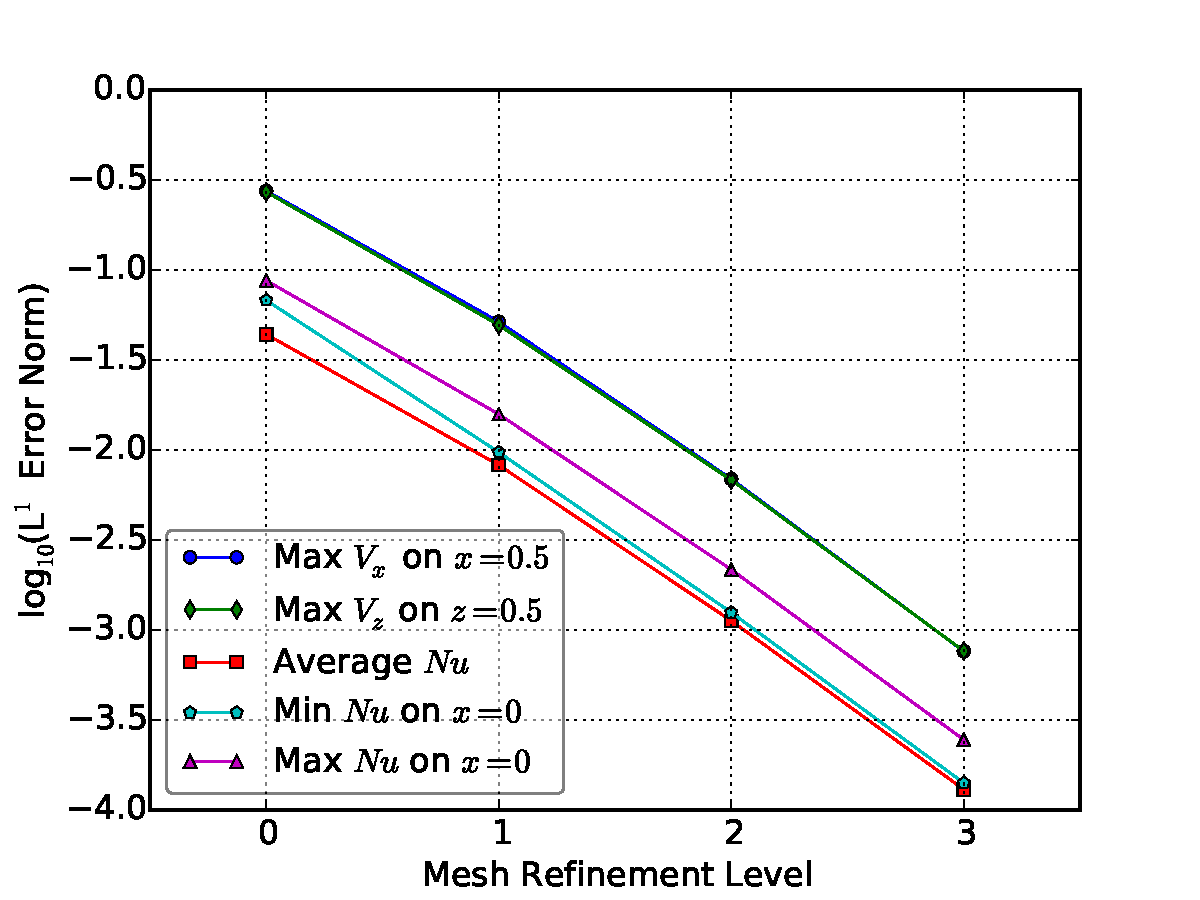
\includegraphics[width=\linewidth]{figs/Ra1000_mr.pdf}
  \caption{\(Ra=10^3\)}
  \label{fig:mr1}
\end{subfigure}
\begin{subfigure}{0.48\textwidth}
  \centering
  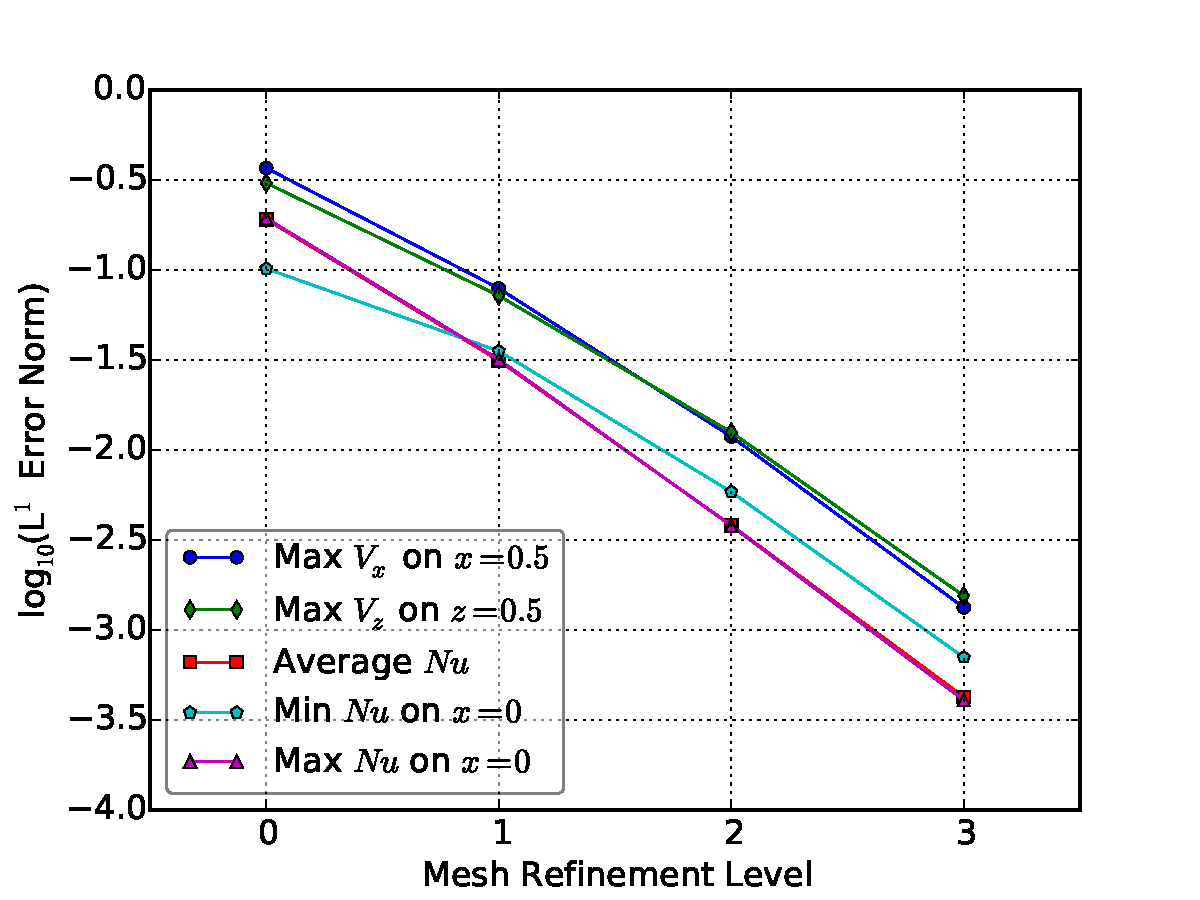
\includegraphics[width=\linewidth]{figs/Ra10000_mr.pdf}
  \caption{\(Ra=10^4\)}
  \label{fig:mr2}
\end{subfigure}
\begin{subfigure}{0.48\textwidth}
  \centering
  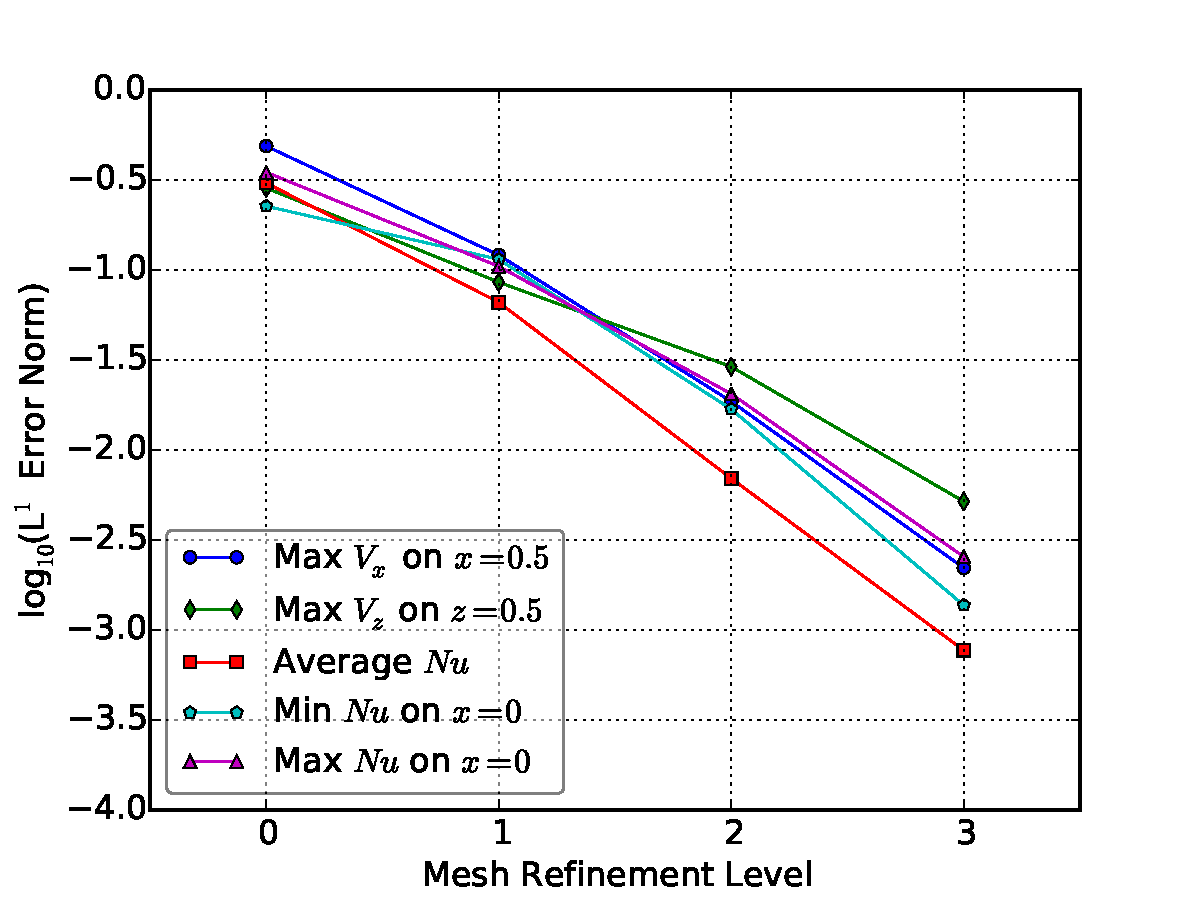
\includegraphics[width=\linewidth]{figs/Ra100000_mr.pdf}
  \caption{\(Ra=10^5\)}
  \label{fig:mr3}
\end{subfigure}
\begin{subfigure}{0.48\textwidth}
  \centering
  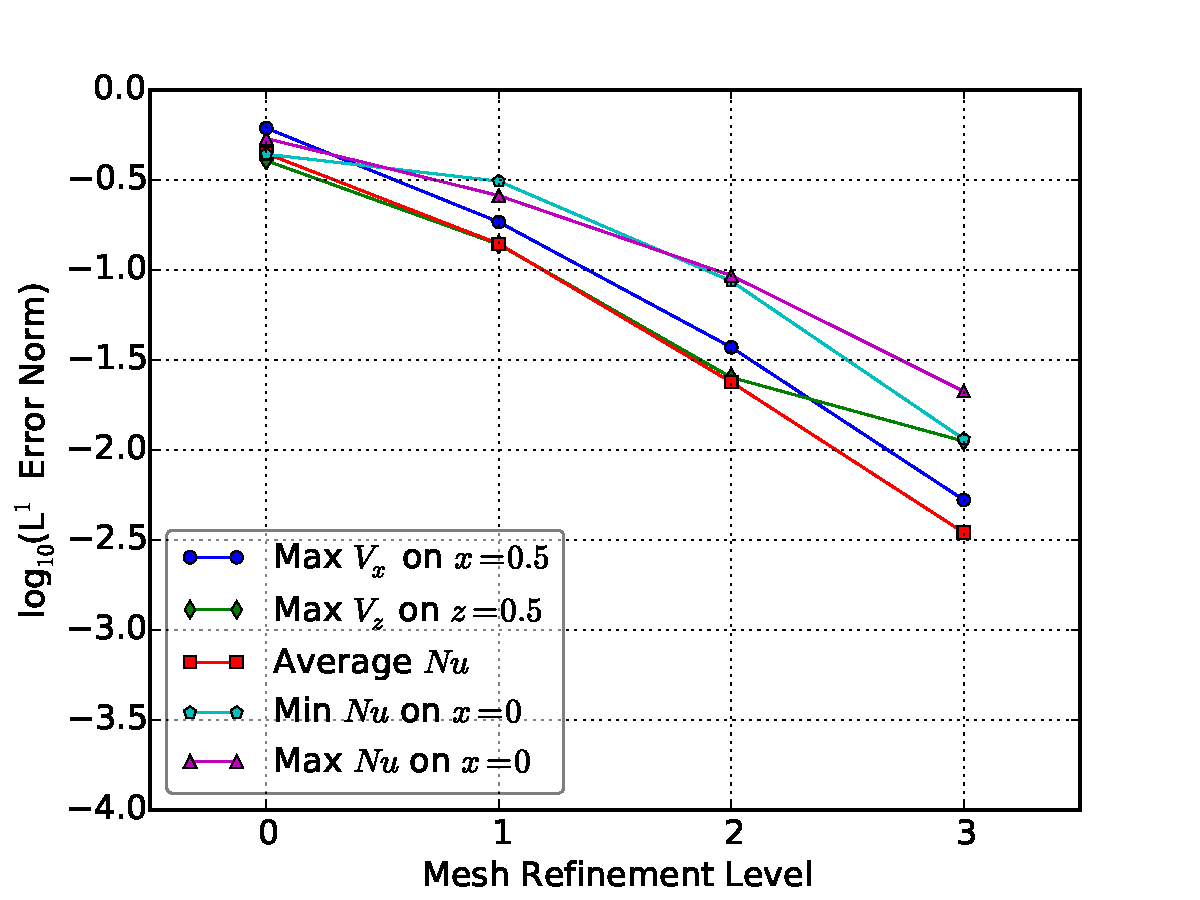
\includegraphics[width=\linewidth]{figs/Ra1000000_mr.pdf}
  \caption{\(Ra=10^6\)}
  \label{fig:mr4}
\end{subfigure}
\caption{L$^1$ error norm of scalar benchmark metrics as a function of the mesh refinement.}
\label{fig:mr}
\end{figure}

Fig.\ \ref{fig:rb_results} shows Pronghorn predictions of fluid temperature, \(x\)-direction velocity, and \(z\)-direction velocity with contours in white for Rayleigh numbers of \(10^3\), \(10^4\), \(10^5\), and \(10^6\). For all cases, the decrease in density along the hot surface causes the fluid to rise along the left wall, while the increase in density along the cool surface causes the fluid to sink along the right wall. 

As the Rayleigh number increases, the thickness of the thermal boundary layer on the hot and cool surfaces becomes thinner, the fluid motion becomes more chaotic, and the heat flux between the vertical cavity walls increases. For higher Rayleigh numbers, the largest \(z\)-velocity magnitudes occur in thinner regions near the vertical walls, while the increased momentum of the vertical flows causes the regions of large \(x\)-velocity magnitudes to move closer to the corners of the cavity.

\begin{figure}[!h]
\centering
\begin{subfigure}{0.32\textwidth}
  \centering
  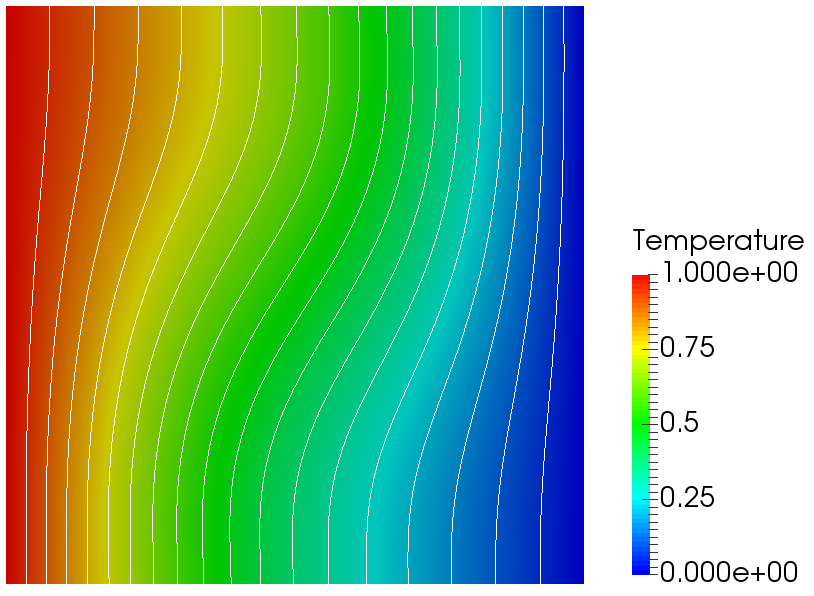
\includegraphics[width=\linewidth]{figs/Ra3_t.png}
  \caption{\(T_f^+\), \(Ra=10^3\)\color{white}1234}
    \vspace*{0.5em}
\end{subfigure}
\begin{subfigure}{0.32\textwidth}
  \centering
  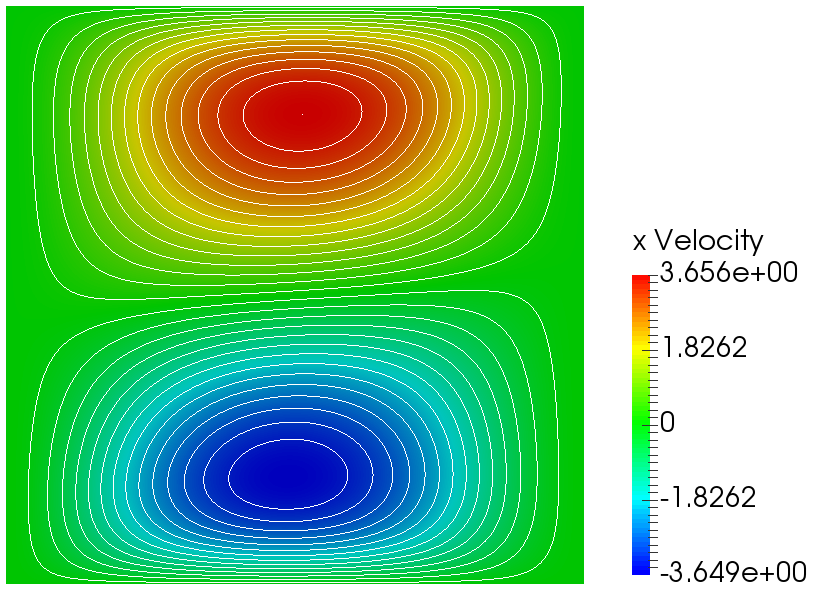
\includegraphics[width=\linewidth]{figs/Ra3_u.png}
  \caption{\(V_x^+\), \(Ra=10^3\)\color{white}1234}
    \vspace*{0.5em}
\end{subfigure}
\begin{subfigure}{0.32\textwidth}
  \centering
  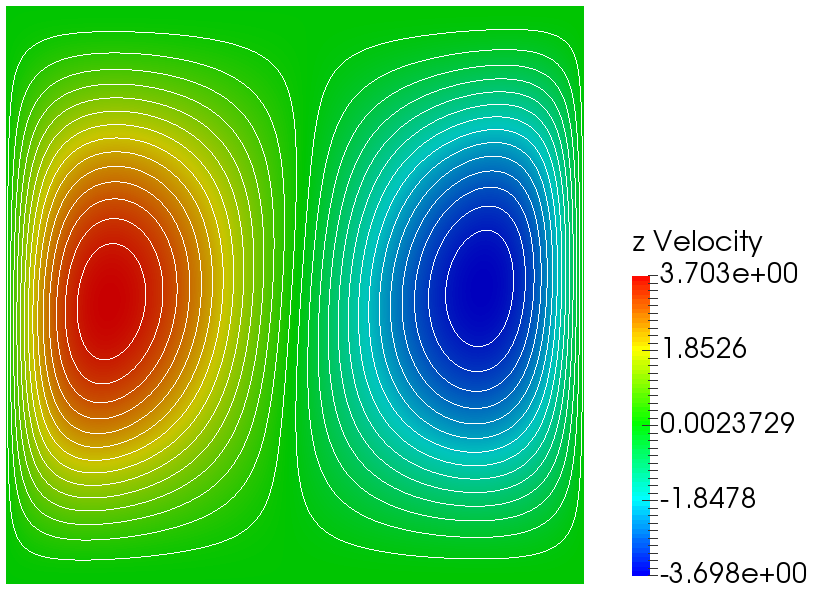
\includegraphics[width=\linewidth]{figs/Ra3_v.png}
  \caption{\(V_z^+\), \(Ra=10^3\)\color{white}1234}
  \vspace*{0.5em}
\end{subfigure}
\begin{subfigure}{0.32\textwidth}
  \centering
  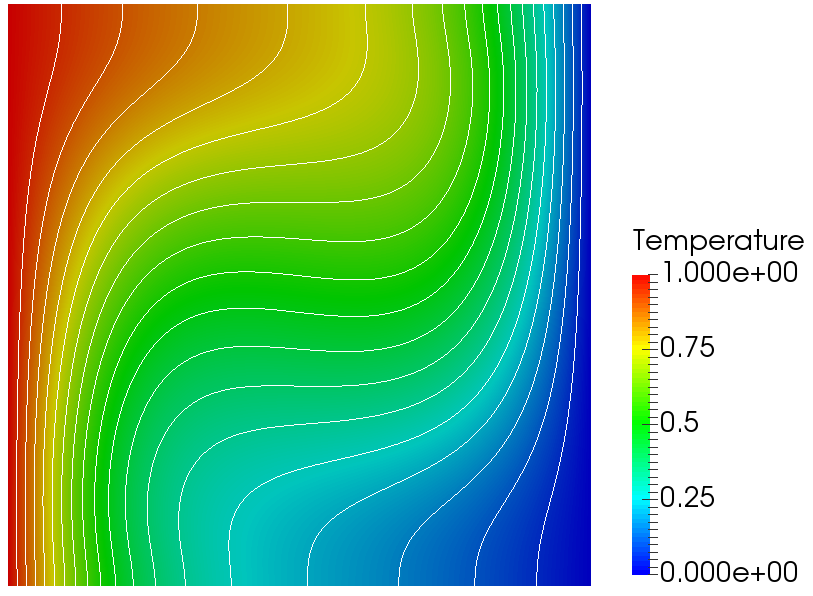
\includegraphics[width=\linewidth]{figs/Ra4_t.png}
  \caption{\(T_f^+\), \(Ra=10^4\)\color{white}1234}
    \vspace*{0.5em}
\end{subfigure}
\begin{subfigure}{0.32\textwidth}
  \centering
  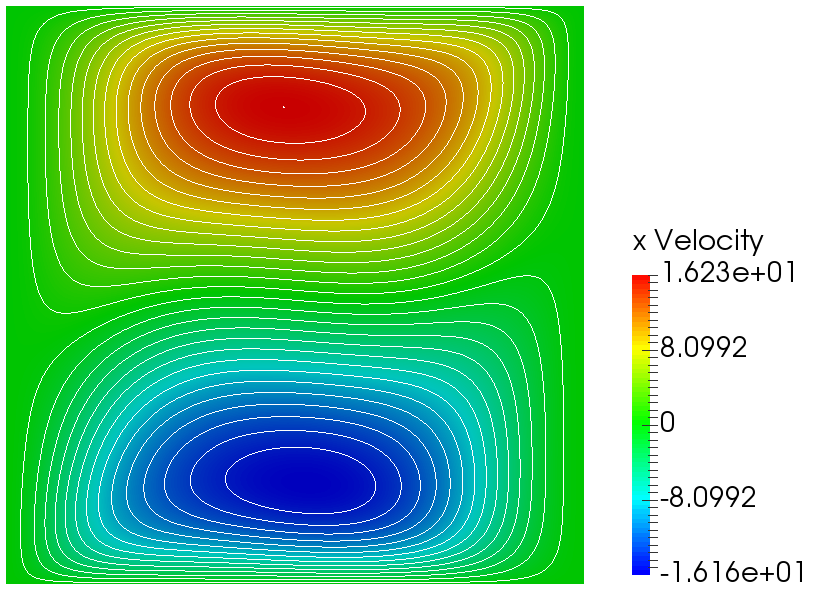
\includegraphics[width=\linewidth]{figs/Ra4_u.png}
  \caption{\(V_x^+\), \(Ra=10^4\)\color{white}1234}
    \vspace*{0.5em}
\end{subfigure}
\begin{subfigure}{0.32\textwidth}
  \centering
  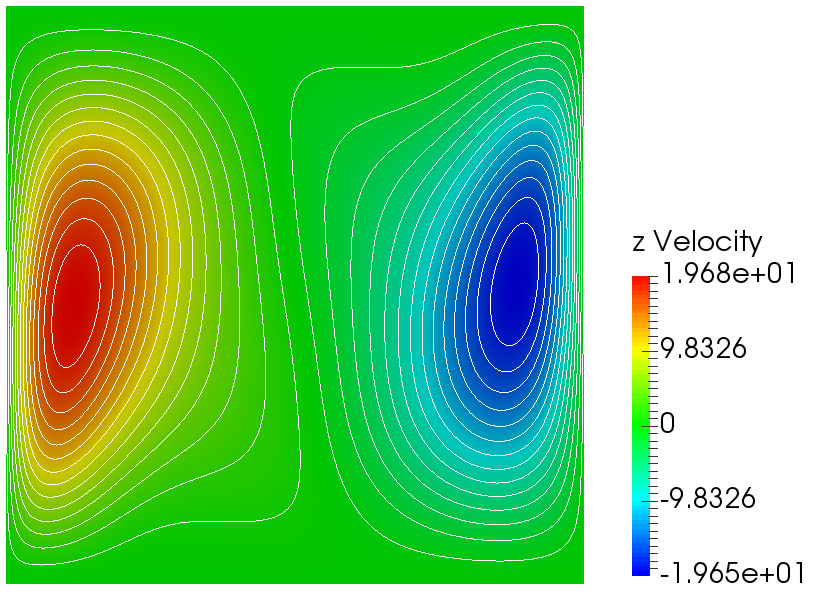
\includegraphics[width=\linewidth]{figs/Ra4_v.png}
  \caption{\(V_z^+\), \(Ra=10^4\)\color{white}1234}
    \vspace*{0.5em}
\end{subfigure}
\begin{subfigure}{0.32\textwidth}
  \centering
  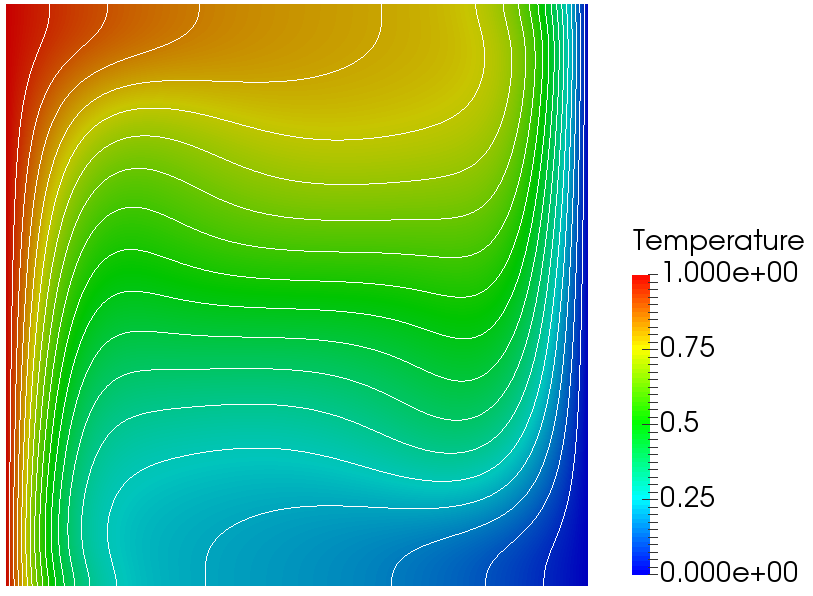
\includegraphics[width=\linewidth]{figs/Ra5_t.png}
  \caption{\(T_f^+\), \(Ra=10^5\)\color{white}1234}
    \vspace*{0.5em}
\end{subfigure}
\begin{subfigure}{0.32\textwidth}
  \centering
  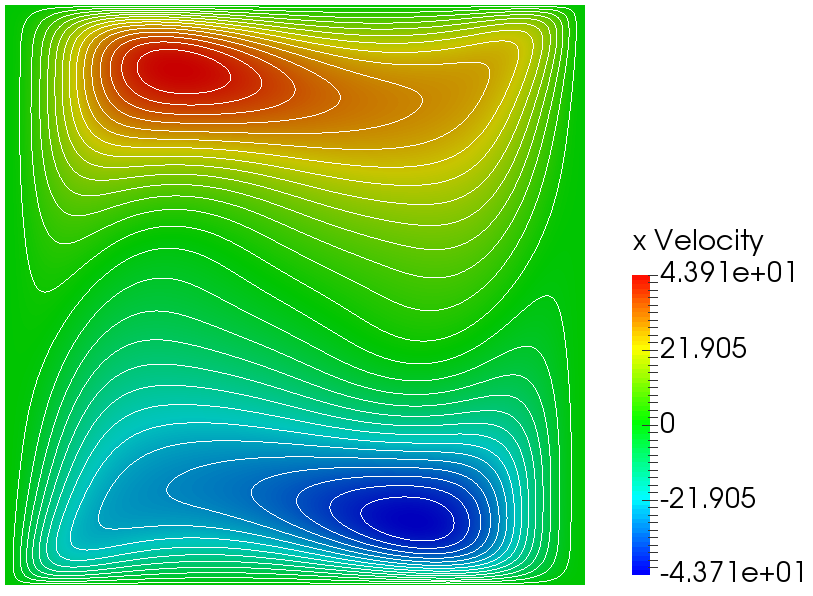
\includegraphics[width=\linewidth]{figs/Ra5_u.png}
  \caption{\(V_x^+\), \(Ra=10^5\)\color{white}1234}
    \vspace*{0.5em}
\end{subfigure}
\begin{subfigure}{0.32\textwidth}
  \centering
  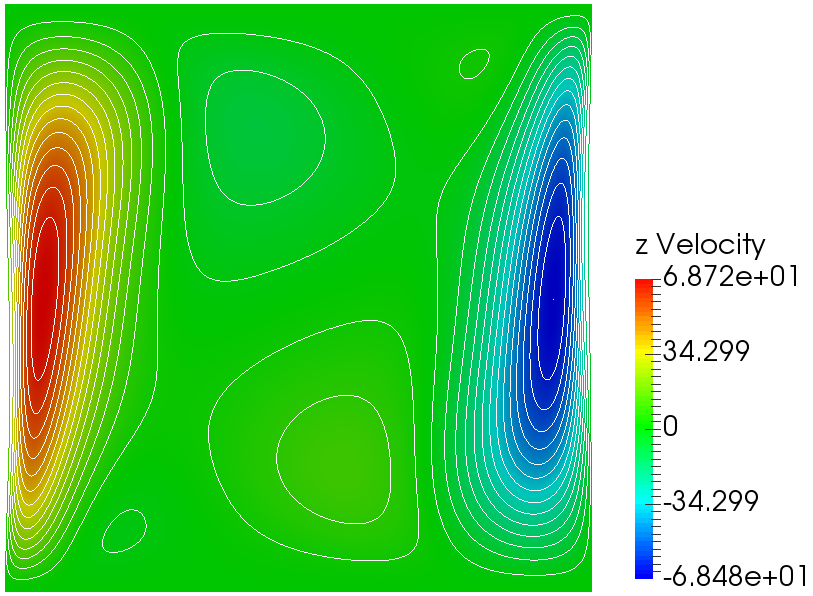
\includegraphics[width=\linewidth]{figs/Ra5_v.png}
  \caption{\(V_z^+\), \(Ra=10^5\)\color{white}1234}
    \vspace*{0.5em}
\end{subfigure}
\begin{subfigure}{0.32\textwidth}
  \centering
  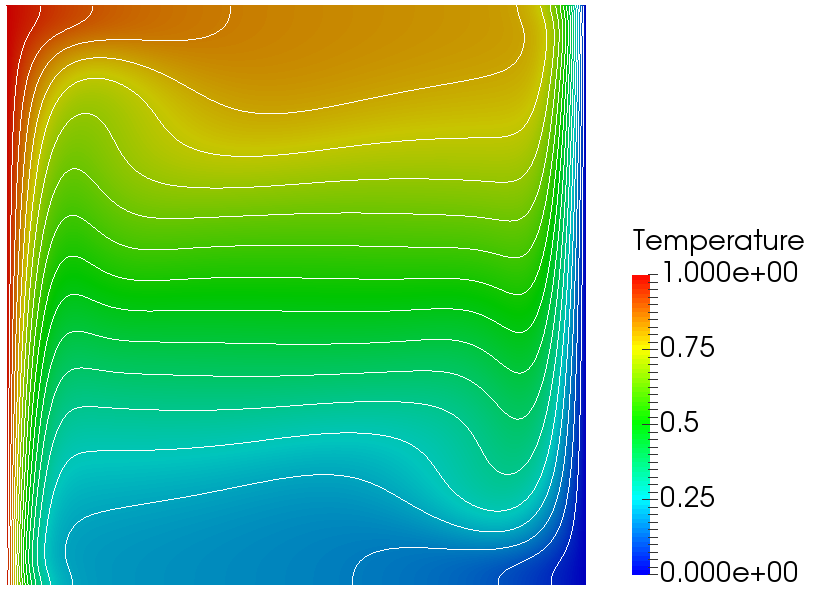
\includegraphics[width=\linewidth]{figs/Ra6_t.png}
  \caption{\(T_f^+\), \(Ra=10^6\)\color{white}1234}
  \label{fig:Ra6T}
    \vspace*{0.5em}
\end{subfigure}
\begin{subfigure}{0.32\textwidth}
  \centering
  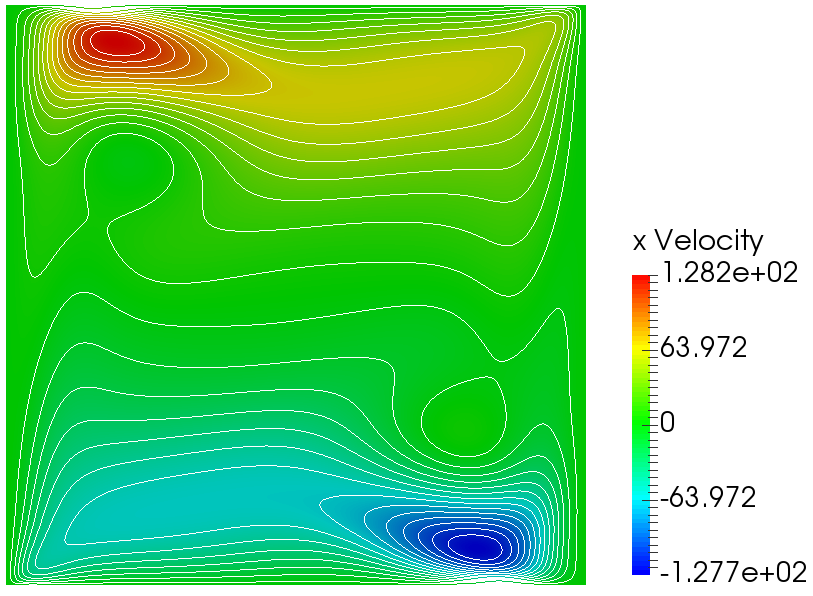
\includegraphics[width=\linewidth]{figs/Ra6_u.png}
  \caption{\(V_x^+\), \(Ra=10^6\)\color{white}1234}
  \label{fig:Ra6u}
    \vspace*{0.5em}
\end{subfigure}
\begin{subfigure}{0.32\textwidth}
  \centering
  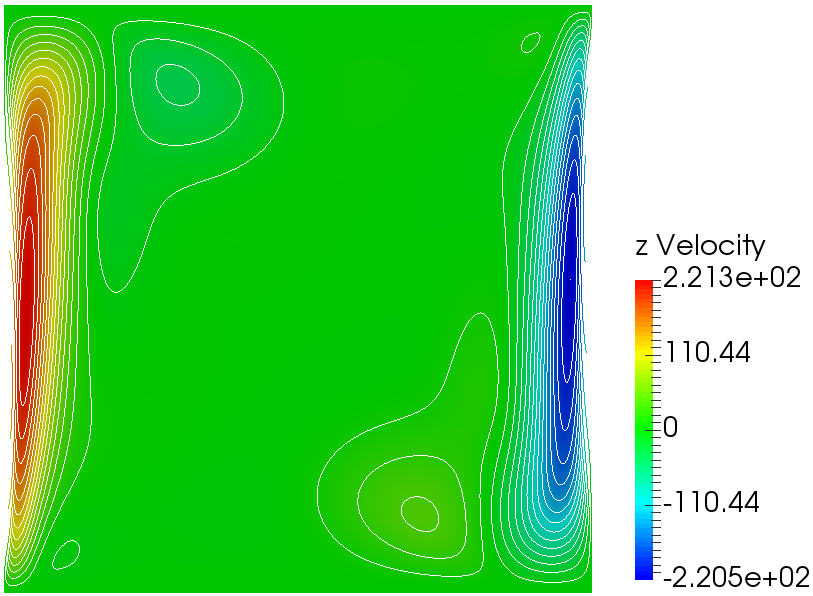
\includegraphics[width=\linewidth]{figs/Ra6_v.png}
  \caption{\(V_z^+\), \(Ra=10^6\)\color{white}1234}
  \label{fig:Ra6v}
    \vspace*{0.5em}
\end{subfigure}
\caption{Pronghorn predictions of \(T_f^+\), \(V_x^+\), and \(V_z^+\) for \mbox{(a -- c)} \(Ra=10^3\), \mbox{(d -- f)} \(Ra=10^4\), \mbox{(g -- i)} \(Ra=10^5\), and \mbox{(j -- l)} \(Ra=10^6\).}
\label{fig:rb_results}
\end{figure}

Table \ref{table:rb} provides a quantitative comparison between the Pronghorn and reference solutions for the scalar benchmark metrics. Given the limited significant figures reported in the benchmark, some relative errors are zero. For most data points, Pronghorn agrees with the reference solution to less than 1\% relative error. The largest relative errors, observed in the predictions for \(z^+_\text{max}\), represent absolute errors on the order of 0.001. When expressed in dimensional form with Eq.\ \eqref{eq:nondim_x}, the absolute error in this \(z_\text{max}\) for \(L=1\) \si{\meter} is only 1 \si{\milli\meter}.

\begin{table}[!h]
\caption{Pronghorn (PH) and reference (Ref.) solutions for the natural convection benchmark \cite{davis_1983} with percent error (Err.) between Pronghorn and the reference.} 
\centering
\footnotesize
\centerline{
\begin{tabular}{|c|c c >{\bfseries}c |c c >{\bfseries}c| c c >{\bfseries}c| c c >{\bfseries}c|}
\hline\hline
 & \multicolumn{3}{c|}{\color{white}${\rvert^\dagger}^\dagger$\color{black}\(Ra=10^3\)\color{white}${\rvert^\dagger}^\dagger$\color{black}} & \multicolumn{3}{c|}{\(Ra=10^4\)} &  \multicolumn{3}{c|}{\(Ra=10^5\)} &  \multicolumn{3}{c|}{\(Ra=10^6\)}\Bstrut\\\cline{2-13}
 & Ref. & PH & Err. & Ref. & PH & Err. & Ref. & PH & Err. & Ref. & PH & Err.\Tstrut\Bstrut\\
\hline
\(V^+_{x,\text{max}}\) & 3.649 & 3.651 & 0.05 & 16.178 & 16.210 & 0.20 & 34.730 & 34.864 & 0.39 & \color{white}0\color{black}64.630 & \color{white}0\color{black}64.780 & 0.23\Tstrut\\
\(z_u^+\) & 0.813 & 0.812 & 0.12 & \color{white}0\color{black}0.823 & \color{white}0\color{black}0.823 & 0.00 & \color{white}0\color{black}0.855 & \color{white}0\color{black}0.855 & 0.00 & \color{white}00\color{black}0.850 & \color{white}00\color{black}0.852 & 0.23\Bstrut\\
\hline
\(V^+_{z,\text{max}}\) & 3.697 & 3.699 & 0.05 & 19.617 & 19.635 & 0.09 & 68.590 & 68.719 & 0.19 & 219.36\color{white}0\color{black} & 220.64\color{white}0\color{black} & 0.58\Tstrut\\
\(x_v^+\) & 0.178 & 0.180 & 1.12 & \color{white}0\color{black}0.119 & \color{white}0\color{black}0.120 & 0.84 & \color{white}0\color{black}0.066 & \color{white}0\color{black}0.066 & 0.00 & \color{white}00\color{black}0.038 & \color{white}00\color{black}0.038 & 0.00\Bstrut\\
\hline
\(\la Nu\ra\) & 1.118 & 1.118 & 0.00 & \color{white}0\color{black}2.243 & \color{white}0\color{black}2.245 & 0.09 & \color{white}0\color{black}4.519 & \color{white}0\color{black}4.519 & 0.00 & \color{white}00\color{black}8.800 & \color{white}00\color{black}8.827 & 0.31\Tstrut\\
\(Nu_\text{min}\) & 0.692 & 0.693 & 0.14& \color{white}0\color{black}0.586 & \color{white}0\color{black}0.588 & 0.34 & \color{white}0\color{black}0.729 & \color{white}0\color{black}0.731 & 0.27 & \color{white}00\color{black}0.989 & \color{white}00\color{black}0.981 & 0.81\\
\(z^+_\text{min}\) & 1.000 & 1.000 & 0.00 & \color{white}0\color{black}1.000 & \color{white}0\color{black}1.000 & 0.00 & \color{white}0\color{black}1.000 & \color{white}0\color{black}1.000 & 0.00 & \color{white}00\color{black}1.000 & \color{white}00\color{black}1.000 & 0.00\\
\(Nu_\text{max}\) & 1.505 & 1.505 & 0.00 & \color{white}0\color{black}3.528 & \color{white}0\color{black}3.532 & 0.11 & \color{white}0\color{black}7.717 & \color{white}0\color{black}7.725 & 0.10 & \color{white}0\color{black}17.925 & \color{white}0\color{black}17.480 & 2.48\\
\(z^+_\text{max}\) & 0.092 & 0.090 & 2.17 & \color{white}0\color{black}0.143 & \color{white}0\color{black}0.144 & 0.70 & \color{white}0\color{black}0.081 & \color{white}0\color{black}0.082 & 1.23 & \color{white}00\color{black}0.038 & \color{white}00\color{black}0.041 & 7.89\Bstrut\\
\hline
\end{tabular}
}
\label{table:rb}
\end{table}

The excellent agreement with the reference benchmark solution demonstrates the capacity of the Navier-Stokes macroscale model to simulate open natural convection flows, providing important verification for the modeling of depressurized conduction cool-down in gas-cooled \glspl{pbr} in Chapter \ref{sec:sana}.

\section{Inviscid Flow Over a Cylinder}
\label{sec:potential_flow}

Because statements of momentum conservation that include the deviatoric viscous stress tensor are often combined with no-slip velocity \glspl{bc} on solid surfaces, the Navier-Stokes model is characterized by thin boundary layers that require enormous element counts and frequently, computationally prohibitive run times to resolve. However, most gas-cooled \glspl{pbr} operate at high Reynolds number such that inertial momentum transport dominates diffusive momentum transport. Because frictional momentum losses are still considered through the distributed loss term \(W\rho_f\vec{V}\), omitting the deviatoric stress tensor is a reasonable simplification to momentum conservation in high-Reynolds-number porous flows that results in more tractable boundary layer meshing requirements \cite{kececioglu}. Omission of the \(-\nabla\cdot(\tilde{\mu}\nabla\vec{V})\) kernel results in flows with significantly different mathematical and physical character to warrant additional verification exercises beyond the viscous convection flow considered in Section \ref{sec:natural_convection}.

This section presents Pronghorn simulations of inviscid flow over a cylinder to verify applicability of the inviscid variation of the Navier-Stokes macroscale model, referred to here as the ``Euler'' macroscale model for brevity, to open flows. This verification exercise is relevant to the use of coarse mesh tools for simulation of effectively \gls{1d} fluid flow in riser channels in \gls{pbr} reflectors and mixing and thermal striping in the open plena adjacent to many \gls{pbr} beds. 

The problem geometry is shown in Fig.\ \ref{fig:pf_geometry}. The cylinder radius \(R\) is 0.25 \si{\meter}. The top, bottom, and cylinder surface boundaries are modeled as insulated slip walls; the left boundary is an inlet with uniform inflow condition

\beq
\label{eq:FreeStreamV}
\vec{V}=U\vec{e}_x\ ;
\eeq

\noindent and the right boundary is a free outlet. The domain width \(W\), height \(H\), and distance from entrance to the cylinder center \(L\) are selected based on recommendations by Hoffman et.\ al to introduce a small distortion from the free-stream velocity \(U\) at the top and bottom boundaries \cite{hoffman_2011}. The fluid is modeled with the Euler macroscale model in Eq.\ \eqref{eq:PorousEquations} with \(\epsilon=1\), \(W=0\), \(\tilde{\mu}=0\), \(\alpha=0\), \(\kappa_f=0\), and \(\kappa_s=0\) and properties closed by the ideal gas \gls{eos}. Further, gravitational acceleration effects are neglected by setting \(\vec{g}=\vec{0}\). The inlet temperature is 300 \si{\kelvin} and the outlet pressure is 1 atm. All \glspl{ic} are uniform and correspond to the inlet temperature and outlet pressure.

\begin{figure}[!h]
\centering
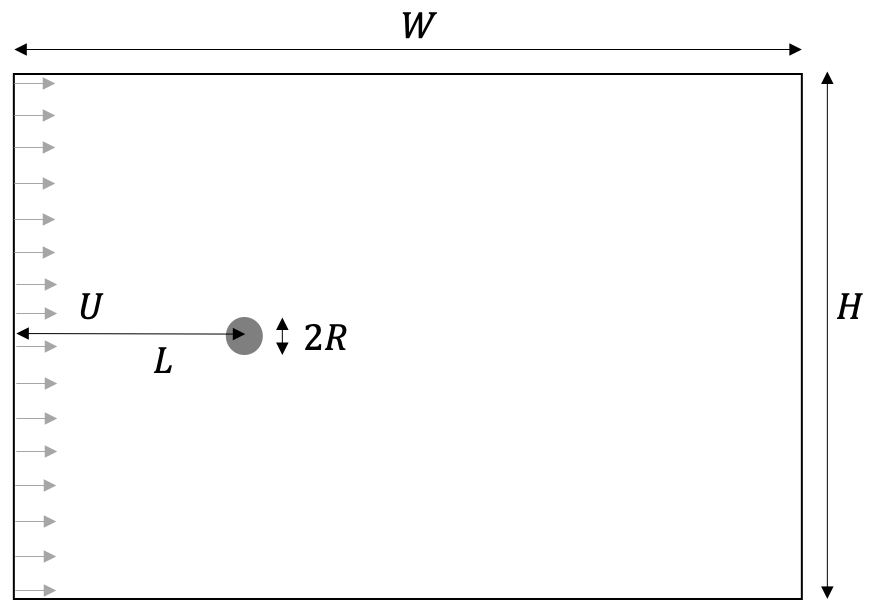
\includegraphics[width=0.5\linewidth]{figs/pf_geometry.png}
\caption{Problem set-up for flow over a cylinder in a rectangular enclosure.}
\label{fig:pf_geometry}
\end{figure}

This particular problem is selected to verify the Euler model because many other canonical Euler flows contain shocks that are not accurately captured with the numerical discretization described in Chapter \ref{sec:ph} due to a lack of ``shock-capturing'' terms \cite{hughes_1986,tezduyar_1986}. In addition, an analytic incompressible potential flow exists for comparison at low Mach numbers where compressibility effects\mdash the only underlying difference between a compressible Euler model and an incompressible potential flow model for the problem in Fig.\ \ref{fig:pf_geometry}\mdash are small. After outlining the potential flow solution, comparisons are made between Pronghorn's compressible Euler model and the incompressible potential flow solution for several different Mach numbers to illustrate that the compressible Euler solution tends towards the analytic incompressible solution as compressibility effects diminish.

The potential flow equations are a simplification to the Euler model for irrotational flow, or flows with zero vorticity \cite{munson,hirsch}. Irrotational flow is automatically satisfied if the velocity can be expressed as the gradient of a scalar potential \(\phi\),

\beq
\label{eq:PotentialVelocity}
\vec{V}=\nabla\phi\ ,
\eeq

\noindent because the curl of a gradient of a scalar is zero. For steady flow, substituting Eq.\ \eqref{eq:PotentialVelocity} into the incompressible Euler mass conservation equation gives a Laplace equation for the potential,

\beq
\label{eq:LaplacePhi}
\nabla^2\phi=0\ .
\eeq

\noindent For flow past a \gls{2d} cylinder, an analytic solution to Eq.\ \eqref{eq:LaplacePhi} is formed by superimposing the solution for uniform inflow with the solution for a doublet, a combination of a source and sink of equal strength separated by a finite distance. A derivation of this solution is available in many introductory fluid mechanics texts \cite{munson}. For a cylinder centered on the origin, the \(x\)- and \(y\)-velocity components are

\beq
\label{eq:V1Analytic}
V_{x,p}=U\left\lbrack1-R^2\frac{x^2-y^2}{(x^2+y^2)^2}\right\rbrack\ ,
\eeq

\beq
\label{eq:V2Analytic}
V_{y,p}=-2UR^2\frac{xy}{(x^2+y^2)^2}\ ,
\eeq

\noindent where a \(p\) subscript is used to denote the potential flow solution. The Bernoulli equation is a simplification of the Euler momentum conservation equation for steady, irrotational, and isentropic flow. Because the \glspl{ic} are uniform, the potential flow model corresponds to isentropic flow. The Bernoulli equation for \(\vec{g}=\vec{0}\) is

\beq
\label{eq:B1}
\nabla\left(\frac{1}{2}V_iV_i+\frac{P}{\rho_f}\right)=0\ .
\eeq

\noindent To obtain the solution for pressure, apply Eq.\ \eqref{eq:B1} at the free-stream conditions of \(\vec{V}=U\vec{e}_x\) and \(P=P_\infty\) in combination with the velocity solutions in Eqs.\ \eqref{eq:V1Analytic} and \eqref{eq:V2Analytic} to give

\beq
\label{eq:PPressure}
P_p=P_\infty+\frac{1}{2}\rho_f\left(U^2-V_iV_i\right)\ .
\eeq

\begin{comment}
\noindent The surface pressure coefficient \(C_P\) represents a normalized pressure and is defined as

\beq
\label{eq:CPDef}
C_P\equiv\frac{P_\text{surface}-P_\infty}{\frac{1}{2}\rho_fU^2}\ .
\eeq

\noindent Substituting the pressure distribution in Eq.\ \eqref{eq:PPressure} with \(x^2+y^2=R^2\) into Eq.\ \eqref{eq:CPDef} gives the surface pressure coefficient for the potential flow as

\beq
\label{eq:PressureCoefficient}
C_{P,p}=1-4\sin^2(\theta)\ ,
\eeq

\noindent where \(\theta\) is the angle relative to the front of the cylinder. 
\end{comment}

\noindent Eqs.\ \eqref{eq:V1Analytic}, \eqref{eq:V2Analytic}, and \eqref{eq:PPressure}, are referred to here as the ``potential flow solution.''

The Mach number \(Ma\) is defined as

\beq
\label{eq:MaDef}
Ma\equiv\frac{\|\vec{V}\|}{c}\ 
\eeq

\noindent and represents the proximity of the flow to supersonic conditions. By writing the stagnation pressure as a Taylor series in terms of the Mach number for an ideal gas, compressibility effects are small for Mach numbers less than about 0.3. Therefore, in the limit of zero Mach number, Pronghorn's compressible Euler solution should predict velocities and pressures that match the potential flow solution. However, a flow simulation at exactly zero Mach number would correspond to a stagnant fluid for which matching the nonzero velocities in Eqs.\ \eqref{eq:V1Analytic} and \eqref{eq:V2Analytic} would not be possible. Therefore, the objective of comparing the compressible Euler solution with the incompressible potential flow solution is only to show that the difference between the two solutions decreases as the Mach number decreases. This investigation verifies both 1)~correct numerical implementation of the inviscid form of the Navier-Stokes macroscale model and 2)~the mechanically compressible dependence on the fluid \gls{eos}.

Three different values of the Mach number are considered\mdash 0.08, 0.16, and 0.32. Each Mach number is a factor of two larger than the next-smallest value, and a Mach number of 0.32 is just above the classically-quoted value of 0.3 below which compressibility effects are insignificant.

A number of different metrics are used to assess the difference between the compressible Euler and incompressible potential flow solutions. The relative L$^2$ norm of the $x$-velocity, $y$-velocity, and pressure are evaluated over the entire domain and are represented as \(\|V_x-V_{x,p}\|/\|V_{x,p}\|\), \(\|V_y-V_{y,p}\|/\|V_{y,p}\|\), and \(\|P-P_p\|/\|P_p\|\), respectively. From Eqs.\ \eqref{eq:V1Analytic} and \eqref{eq:V2Analytic}, the potential flow velocity at the top of the cylinder is \(2U\). While the three norms listed earlier are computed over the entire domain, a point indicator of the velocity difference is useful for assessing error contributions due to the finite geometry. Therefore, the relative difference in the velocity at the top of the cylinder is included and represented as \(|V_x(0, R)-2U|/2U\).

A mesh refinement study is performed for the largest Mach number of 0.32 in the same fashion as in Section \ref{sec:natural_convection}. A starting mesh is uniformly refined until the relative change in the three L$^2$ norms described in the preceding paragraph is less than 5\% between two successive meshes. The finer of these two meshes is then used for all other Mach numbers.

First, a quantitative comparison between Pronghorn's compressible Euler model and the incompressible potential flow solution is provided. Table \ref{table:MNerror} summarizes the difference between the two models as a function of the Mach number. As expected, the difference between Pronghorn's compressible Euler solution and the incompressible potential flow solution decreases as the Mach number decreases.

\begin{table}[!h]
\caption{Difference between Pronghorn's compressible Euler solution and the incompressible potential flow solution as a function of the Mach number.}
\centering
\begin{tabular}{|c |c c c c|}
\hline\hline
\(Ma\) & \(\|V_x-V_{x,p}\|/\|V_{x,p}\|\) & \(\|V_y-V_{y,p}\|/\|V_{y,p}\|\) & \(|V_{x}(0, R)-2U|/2U\) & \(\|P-P_p\|/\|P_p\|\)\Tstrut\Bstrut\\
\hline
0.08 & \(3.53\times10^{-3}\) & \(3.27\times10^{-2}\) & \(2.62\times10^{-3}\) & \(1.50\times10^{-5}\)\Tstrut\\
0.16 & \(3.60\times10^{-3}\) & \(3.70\times10^{-2}\) & \(1.91\times10^{-2}\) & \(7.29\times10^{-5}\)\\
0.32 & \(4.88\times10^{-3}\) & \(8.48\times10^{-2}\) & \(8.72\times10^{-2}\) & \(6.71\times10^{-4}\)\Bstrut\\
\hline
\end{tabular}
\label{table:MNerror}
\end{table}

For the L$^2$ norms computed over the entire domain, or the second, third, and fifth columns in Table \ref{table:MNerror}, the reduction in these norms when halving the Mach number from 0.32 to 0.16 is much larger than the reduction when halving the Mach number from 0.16 to 0.08. For instance, the relative \(x\)-velocity norm decreases by a factor of 1.35 when halving the Mach number from 0.32 to 0.16, while only decreasing by a factor of 1.02 when halving the Mach number from 0.16 to 0.08. This occurs because of the finite size of the domain. That is, the difference in the two solutions should not be expected to tend to zero in the limit of zero Mach number\mdash the top and bottom walls are streamlines in the compressible Euler model, while the potential flow solution was derived with free stream \glspl{bc} as \(x, y\rightarrow\infty\) that result in nonzero curvature at \(y=\pm H/2\). To more clearly see this effect, consider the pointwise difference in the $x$-velocity at the top of the cylinder, which is sufficiently far from boundaries as to be unaffected by the \(W\) and \(H\) dimensions. In halving the Mach number from 0.32 to 0.16 and from 0.16 to 0.08, the relative difference in the $x$-velocity at the top of the cylinder decreases by a factor of 4.56 and 7.29, respectively. No significantly reduced solution difference is observed as the Mach number decreases for this pointwise metric.

The implicit \gls{bc} on the upper boundary does not impose any free-stream pressure such that the relative difference in the pressure distributions is comparatively unaffected by the finite nature of the domain. The relative difference in the pressure decreases by a factor of 9.20 as the Mach number is halved from 0.32 to 0.16 and by a factor of 4.79 as the Mach number is halved from 0.16 to 0.08.

To conclude this section, Pronghorn predicted velocity and pressure distributions for an inlet Mach number of 0.08 are presented. Define a nondimensional speed \(V^+\) as

\begin{equation}
V^+=\frac{\|\vec{V}\|}{U}\ .
\end{equation}

\noindent For the incompressible potential flow solution, \(V^+\) varies from zero on the front and back sides of the cylinder to 2.0 at the top and bottom of the cylinder. In the region near the cylinder, Fig.\ \ref{fig:Ma08} shows the nondimensional speed and pressure. In the speed subfigure, streamlines are shown as black lines. In the pressure subfigure, contours are shown colored by the pressure. The flow is nearly symmetric about the cylinder. At the front and rear stagnation points, the pressure is highest and the velocity lowest. Flow acceleration around the cylinder results in the highest velocities and lowest pressures occurring on the top and bottom of the cylinder. As already shown by the various norms in Table \ref{table:MNerror}, the velocity and pressure match the incompressible potential flow solution to within 4\% relative difference.

\begin{figure}[!h]
  \centering
  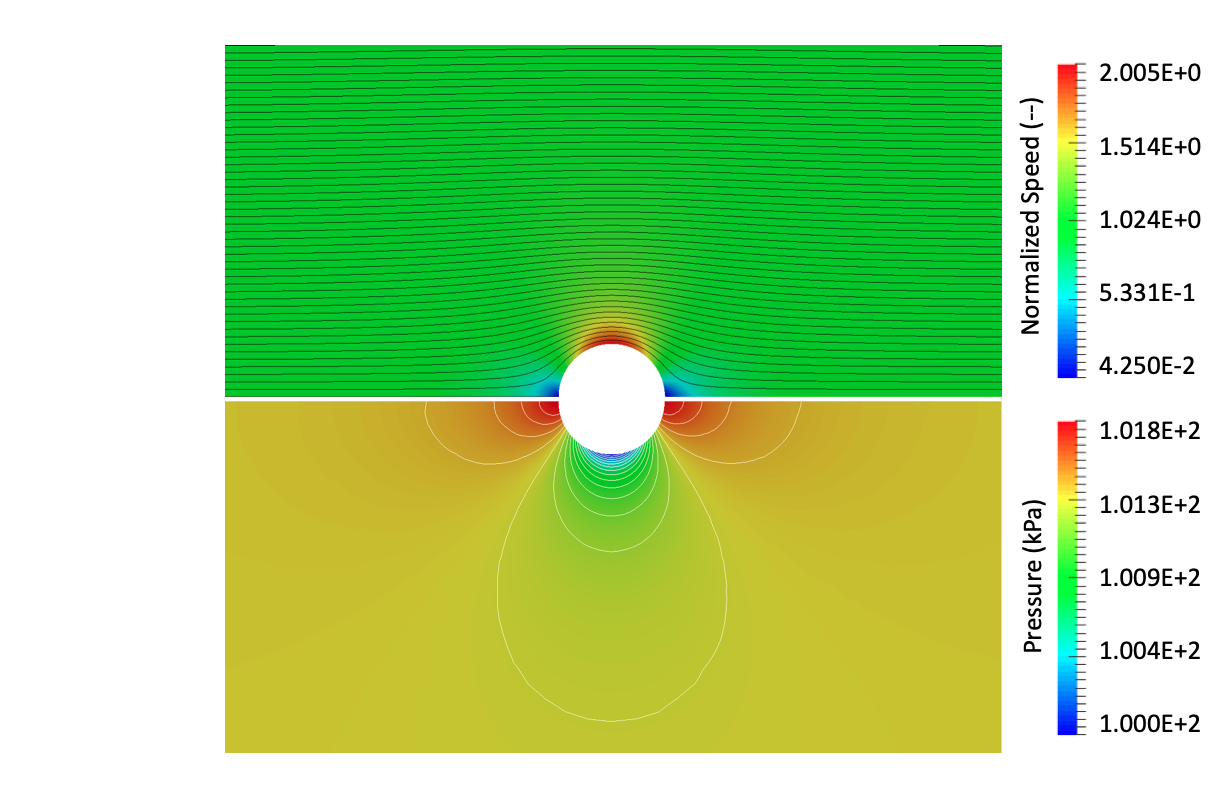
\includegraphics[width=0.7\linewidth]{figs/pf_Ma08.png}
  \caption{Pronghorn predicted \(V^+\), with streamlines in black, and \(P\), with contours shown colored by \(P\), for an inlet Mach number of 0.08.}
  \label{fig:Ma08}
\end{figure}

Overall, the mechanical compressibility effects are correctly modeled with the inviscid Navier-Stokes macroscale model. The combination of 1)~reduced differences between the compressible Euler and incompressible potential flow solutions as the Mach number decreases and 2)~low relative differences for Mach numbers in the range of \(0.08\leq Ma\leq0.32\) demonstrates the capacity of the inviscid Navier-Stokes model to simulate open flows, providing important verification for the modeling of high-Reynolds number flows in \glspl{pbr}.

\section{The Heat Source Decomposition Model}
\label{sec:verification_meso}

Given the computing resources available for routine design and analysis, the heterogeneous nature of \gls{pbr} fuels requires the use of multiscale models to predict temperatures. Simply homogenizing the fission heat source and thermal properties fails to capture the thermal resistance imposed by the low-conductivity buffer layer, and may result in significant underprediction of fuel temperatures. 

Two multiscale models were introduced in Chapter \ref{sec:PhysicalModels}\mdash the \gls{hsd} model and the \gls{hl} model. This section applies the \gls{hsd} model to a Cartesian domain consisting of nine \glspl{cfp} in a matrix and provides a comparison against a fully-resolved heat conduction solution of the same geometry. The objectives of this analysis are to 1)~verify the \gls{hsd} method for a simple, but representative, domain; 2)~explain the microscale ``translation'' process in Eq.\ \eqref{eq:MultiscaleSolution}; and 3)~address the accuracy of the averaging approximation in Eq.\ \eqref{eq:AvgT}. Because the \gls{mms} tests described in Section \ref{sec:mms} verify correct implementation of the diffusion kernels needed for the multi-layer \gls{hl} method, no such dedicated verification is required for the \gls{hl} method, which is simply a multi-layer conduction model.

For this demonstration problem, each \gls{cfp} is composed of five material layers with a uniform heat source of \(2\times10^8\) \si{\watt\per\cubic\meter} in the center kernel. While this power density is higher than that used in most \glspl{pbr}, the larger magnitude is selected to accentuate the differences between the meso and micro scale solutions. The \glspl{cfp} occupy 40\% by volume of the matrix material. Fig.\ \ref{fig:nine_particle_mesha} shows the mesh, colored by material ID, used to obtain the reference temperature solution. The \gls{cfp} layer thicknesses are the same as those in the \gls{pbfhr} design in Table \ref{table:pebble_props} and are typical of most \gls{triso} particle designs. Thermal properties in dimensionally consistent units are shown for each material in Fig.\ \ref{fig:nine_particle_mesha}. Thermal \glspl{bc} are selected to have a significant thermal gradient over the domain. The top, left, and right boundaries are set to 1100\si{\celsius}, 1100\si{\celsius}, and 1150\si{\celsius}, respectively, while the bottom boundary is insulated.

\begin{figure}[!h]
\centering
\hspace{1cm}
  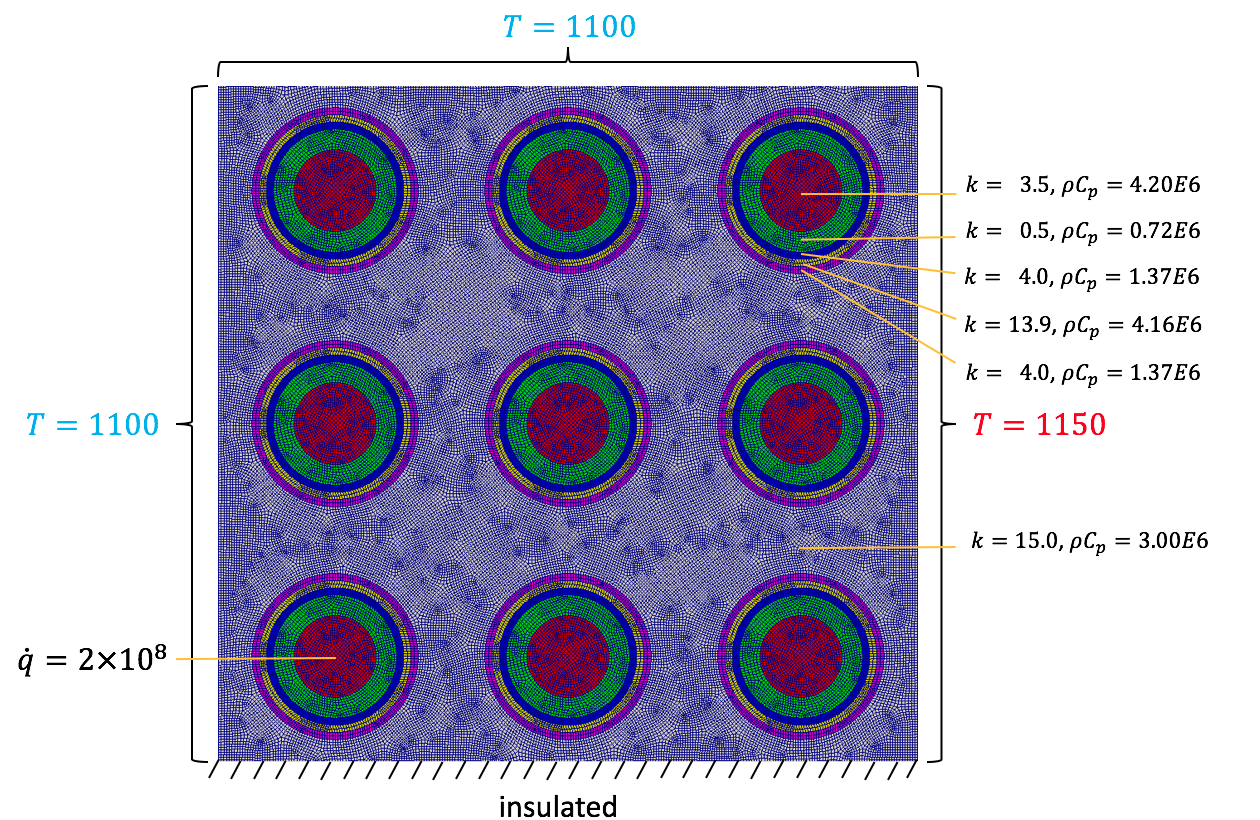
\includegraphics[width=0.75\linewidth]{figs/multiscale_9_problem.png}
\caption{Reference mesh and problem setup for a heterogeneous solid with \glspl{cfp} in a matrix.}
\label{fig:nine_particle_mesha}
\end{figure}

The reference temperature solution, shown in Fig.\ \ref{fig:nine_particle_mesh}, is obtained by solving the heat conduction equation in Eq.\ \eqref{eq:oem} with the \gls{moose} heat conduction module. The temperature contours are tightly packed in the second material layer in each \gls{cfp} due to its relatively low thermal conductivity. The objective of the \gls{hsd} model is to approximate the temperature distribution in Fig.\ \ref{fig:nine_particle_mesh} with significantly lower computational effort.

\begin{figure}[!h]
  \centering
  \hspace{3.2cm}
  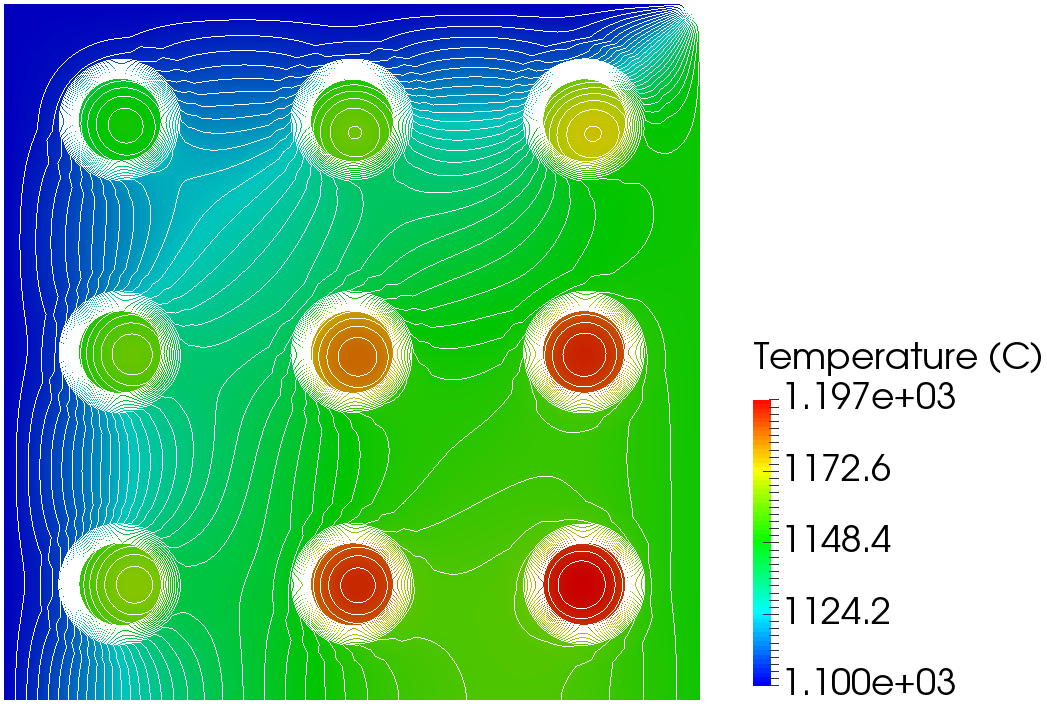
\includegraphics[width=0.63\linewidth]{figs/compact_9_reference.png}
\caption{Reference temperature solution for the mesh in Fig.\ \ref{fig:nine_particle_mesha} with contour lines in white.}
\label{fig:nine_particle_mesh}
\end{figure}

The \gls{hsd} method involves the coupled solutions of the mesoscale model in Eq.\ \eqref{eq:MesoscaleSolution} and the microscale model in Eq.\ \eqref{eq:MicroscaleSolution}. The mesoscale mesh encompasses the entire heterogeneous region and is shown in Fig.\ \ref{fig:nine_particle_mesoscalea}. The \gls{cfp} properties are homogenized with the volume average in Eq.\ \eqref{eq:series}. \(\rho_\text{meso}\), and \(C_{p,\text{meso}}\) are then evaluated with the volume average in Eq.\ \eqref{eq:series}, while \(k_\text{meso}\) is evaluated with the Chiew and Glandt averaging theorem in Eq.\ \eqref{eq:ChiewGlandt}. The volumetric heat source is averaged over the \glspl{cfp} and matrix.

The mesoscale solution is shown in Fig.\ \ref{fig:nine_particle_mesoscaleb}. The mesoscale temperature represents a long-wavelength ``background'' response to the \glspl{bc}, averaged thermal properties, and averaged heat source. Note that the color bar in Fig.\ \ref{fig:nine_particle_mesoscaleb} is intentionally not the same as in Fig.\ \ref{fig:nine_particle_mesh} to reinforce that it is the sum of the meso and micro scale solutions that satisfies the imposed \glspl{bc}.

\begin{figure}[!h]
\centering
\begin{subfigure}{.45\textwidth}
  \centering
  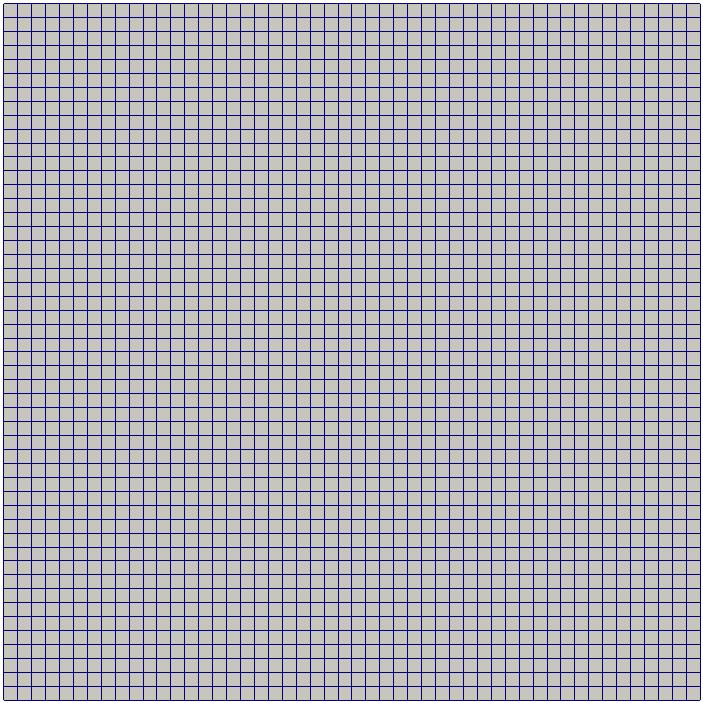
\includegraphics[height=0.72\linewidth]{figs/mesoscale_9_mesh.png}
  \caption{Mesoscale problem}
  \label{fig:nine_particle_mesoscalea}
\end{subfigure}
\begin{subfigure}{.45\textwidth}
  \centering
  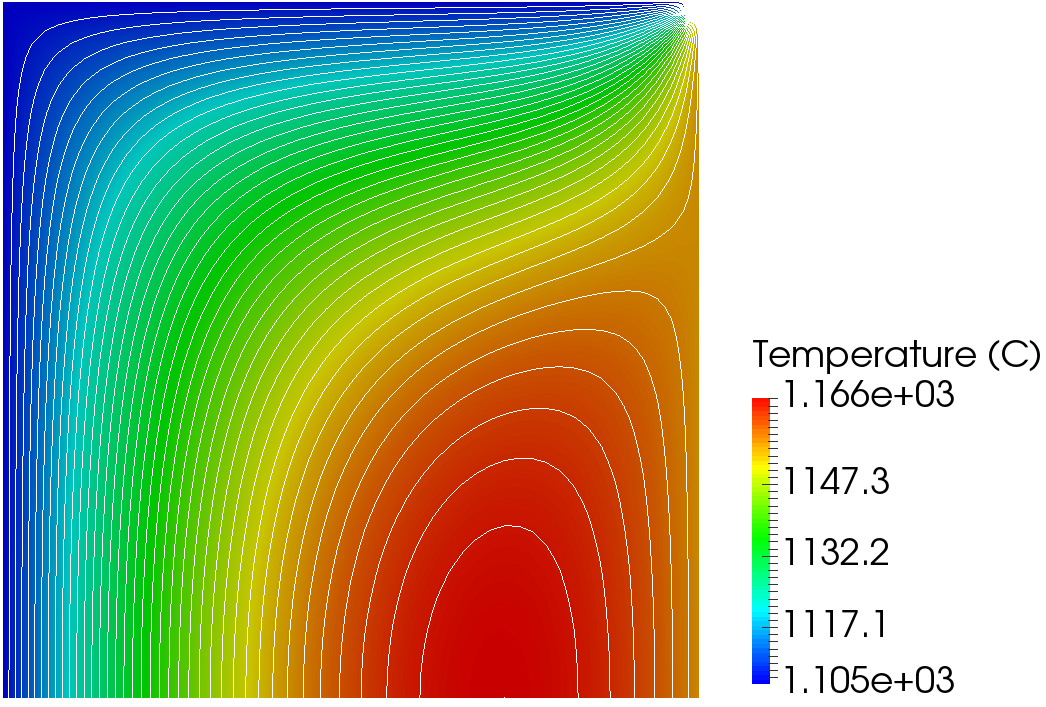
\includegraphics[height=0.71\linewidth]{figs/compact_9_mesoscale.png}
  \caption{Mesoscale solution}
  \label{fig:nine_particle_mesoscaleb}
\end{subfigure}
\caption{\gls{hsd} mesoscale (a) mesh and (b) solution with contour lines in white.}
\label{fig:nine_particle_mesoscale}
\end{figure}

The microscale domain, shown in Fig.\ \ref{fig:micro_a}, is a \gls{1d} representation of a \gls{cfp} plus a layer of matrix material sized to preserve all material \glspl{pf}. \(\rho_\text{micro}\), \(C_{p,\text{micro}}\), and \(k_\text{micro}\) are the local properties shown in Fig.\ \ref{fig:nine_particle_mesha}. The fluctuating heat source is positive within the central kernel and negative in all other regions to preserve the zero average. Fig.\ \ref{fig:micro_b} shows the microscale temperature solution. Because the fluctuating heat source is negative outside the central kernel, the temperature is negative in the outermost regions of the microscale domain.

\begin{figure}[!h]
\centering
\begin{subfigure}[b]{0.49\linewidth}
\centering
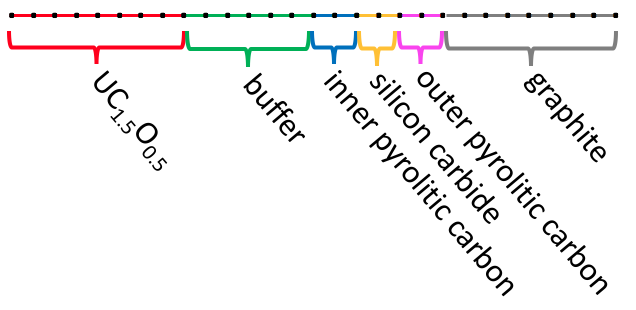
\includegraphics[width=6.cm]{figs/microscale_domain_colored.png}
\vspace{2em}
\caption{Microscale problem}
\label{fig:micro_a}
\end{subfigure}
\begin{subfigure}[b]{0.49\linewidth}
\centering
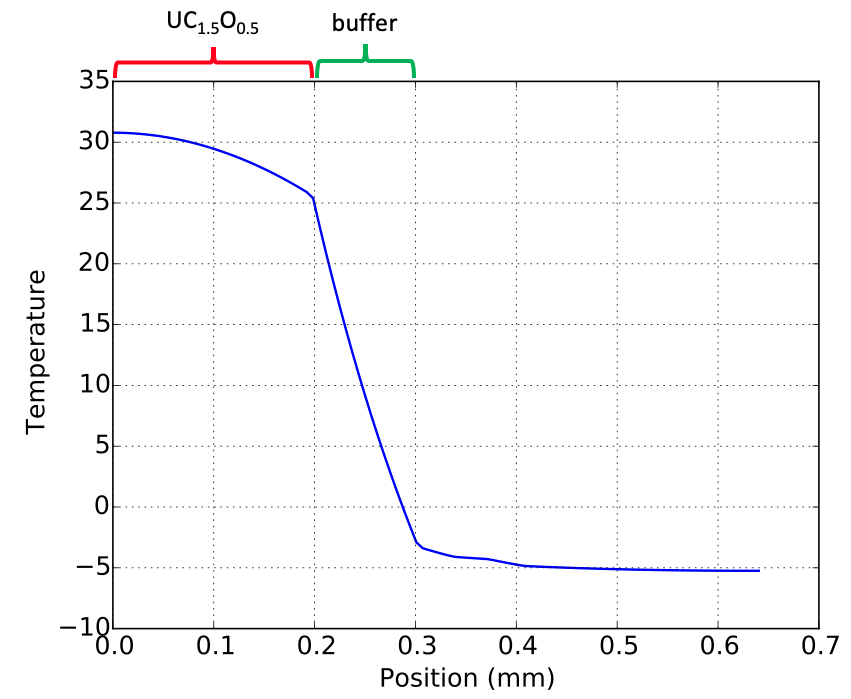
\includegraphics[height=6.cm]{figs/microscale_solution.png}
\caption{Microscale solution}
\label{fig:micro_b}
\end{subfigure}
\caption{\gls{hsd} microscale (a) mesh and (b) solution.}
\end{figure}

Fig.\ \ref{fig:MMD_example} shows the reference and \gls{hsd} solutions along a horizontal line passing through the centers of the middle row of particles. The low-conductivity buffer results in significantly higher kernel temperatures than in surrounding materials. The bottom section of Fig.\ \ref{fig:MMD_example} shows the microscale solution translated to the location of each of the three particles. According to Eq.\ \eqref{eq:MultiscaleSolution}, the \gls{hsd} multiscale approximation is the sum of the long-wavelength mesoscale solution and the translated microscale solutions, and is shown as a red dashed line in Fig.\ \ref{fig:MMD_example}. The \gls{hsd} solution agrees very well with the reference temperature solution; the only source of error in the \gls{hsd} method is the homogenization of the mesoscale properties.

\begin{figure}[!h]
\centering
\includegraphics[width=0.6\linewidth]{figs/nine_center_row_multiscale.png}
\caption{Multiscale, mesoscale, microscale, and reference solutions for the problem in Fig.\ \ref{fig:nine_particle_mesha}.}
\label{fig:MMD_example}
\end{figure}

It is important to note that legacy \gls{pbr} applications that simply homogenize the thermal properties and heat source to represent the fuel temperature with a single heat conduction \gls{pde} can only predict the long-wavelength background temperature in Fig.\ \ref{fig:MMD_example}. Such models would fail to capture the high kernel temperatures resulting from the buffer thermal resistance, and are hence not considered in this work.

Next, in order to verify applicability of the \gls{hsd} method to transients, consider the same problem in Fig.\ \ref{fig:nine_particle_mesha} with a time-dependent heat source given by

\begin{equation}
\label{eq:time_q}
\dot{q}=2\times10^8(t+1)\ .
\end{equation}

\noindent With this heat source, Fig.\ \ref{fig:time_q} shows the reference and \gls{hsd} multiscale solutions along a horizontal line passing through the centers of the middle row of particles. The \gls{hsd} approximation again agrees very well with the reference solution at all times considered. 

\begin{figure}[!h]
\centering
\begin{subfigure}[b]{0.49\linewidth}
\centering
\includegraphics[width=1.1\linewidth]{figs/nine_particle_center_row_transient.png}
\caption{Solutions along line through center particles}
\label{fig:time_q}
\end{subfigure}
\begin{subfigure}[b]{0.49\linewidth}
\centering
\includegraphics[width=1.1\linewidth]{figs/nine_particle_transient_postprocessors.png}
\caption{Solutions averaged in space}
\label{fig:avg_nine}
\end{subfigure}
\caption{Reference (---) and \gls{hsd} multiscale solutions (- -) (a) along a line through the centers of the middle row of particles and (b) spatially-averaged for the problem in Fig.\ \ref{fig:nine_particle_mesha} with the heat source in Eq.\ \eqref{eq:time_q}.}
\end{figure}

Fig.\ \ref{fig:avg_nine} shows the average temperatures of each material as a function of time. To reflect conditions typical of \gls{pbr} analysis, where the \gls{cfp} locations are unknown, the \gls{hsd} averages are evaluated with Eq.\ \eqref{eq:AvgT}. Excellent agreement is observed between the multiscale and reference solutions, especially considering that the mesoscale solution in this particular test problem varies on the order of the micro length scale.

The excellent agreement between the \gls{hsd} model and reference solution demonstrates the capacity of the \gls{hsd} model to simulate heat conduction in heterogeneous solids, providing important verification before application of the \gls{hsd} model to the Mark-1 \gls{pbfhr} in Chapter \ref{sec:pbfhr}.